\chapter{Referencial Teórico}\label{cap:referencias}

% --------------------------------------------------------------------------- %
\section{Considerações Iniciais}

Este capítulo tem como finalidade conceituar teoricamente as aplicações e técnicas que fundamentaram a realização deste trabalho. Serão abordadas as definições de análise de dados e ciência de dados, destacando suas importâncias perante o cenário cientifico e tecnológico, além de conceituar o seu emprego na elaboração e organização de conjuntos de dados como os que nortearam o presente estudo. Também será abordada a importância das bases de dados governamentais disponibilizadas pelos órgãos públicos, finalizando o capítulo com uma fundamentação das técnicas matemáticas aplicadas nesta pesquisa.

% --------------------------------------------------------------------------- %
\section{Análise de Dados}

Com a evolução de novas e mais modernas tecnologias, aliada ao advento da Internet e das mídias sociais, uma enorme quantidade de dados está sendo gerada e coletada diariamente a uma velocidade cada vez maior \cite{cap02_ref7, cap02_ref10}. Celulares, notebooks, equipamentos hospitalares, automóveis, sensores, câmeras de segurança e diversos outros dispositivos eletrônicos presentes nos mais diversos segmentos da sociedade geram automaticamente informações que precisam ser armazenadas e muitas vezes processadas em tempo real. Entretanto, acompanhar, analisar e extrair conhecimento acerca desse fluxo de dados é uma tarefa substancialmente desafiadora, especialmente quando estes não estão em conformidade com as noções tradicionais de estrutura de dados \cite{cap02_ref3}.

Tal fenômeno, além de estar cada vez mais inserido no cotidiano da população, tem apresentado um crescimento exponencial. Segundo \cite{cap02_ref4} aproximadamente 90\% dos dados existentes no mundo foram criados nos últimos 2 anos\footnote{Informações referentes ao ano de 2016.}. Adicionalmente, o barateamento de ferramentas computacionais com maior poder de processamento e a onipresença da rede estão colaborando para que pessoas e empresas desenvolvam algoritmos acerca desses dados nas mais diversas áreas do conhecimento como: economia, engenharia, sociologia, saúde, marketing, dentre outras \cite{cap02_ref9, cap02_ref5}

Diante desse cenário, a utilização de técnicas computacionais para a aquisição inteligente de conhecimento acerca de dados sem representatividade passou a ser uma tarefa cada vez mais atrativa, uma vez que muda a forma como tais dados são analisados e contextualizados \cite{cap02_ref11}. Desse modo, Mineração de Dados (MD), Extração de Conhecimento de Base de Dados (mais conhecida como \textit{Knowledge-Discovery in Database} – KDD) e Inteligência de Negócios (do inglês \textit{Business Inteligence} – BI) são exemplos de métodos ou estratégias que buscam extrair informações e identificar padrões/tendências para a resolução de problemas específicos acerca de conjunto de dados \cite{cap02_ref12, cap02_ref4}. 

Embora diversos autores interpretem os processos KDD e MD como sinônimos \cite{cap02_ref11, cap02_ref6}, boa parte da literatura considera a mineração como uma etapa da descoberta de conhecimento, sendo essa composta pela seleção, pré-processamento, transformação, mineração de dados e interpretação \cite{cap02_ref12, cap02_ref5}. A Figura~\ref{fig:kdd_process} elenca as etapas necessárias para a extração de conhecimento.


\begin{figure}[htpb]
   \centering
   \caption{Processo de descoberta de conhecimento em bases de dados.}
   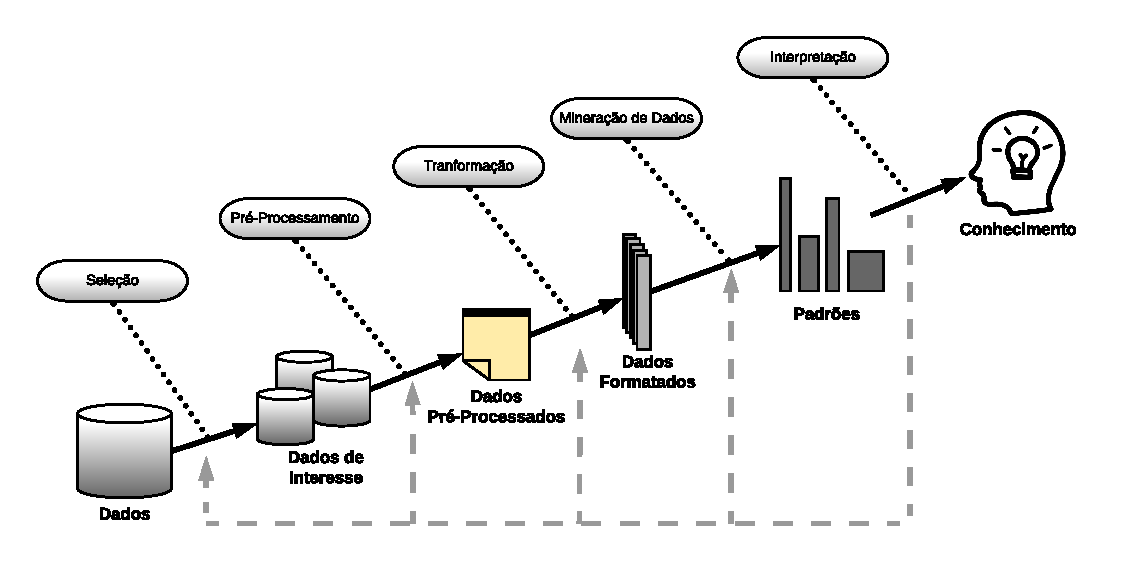
\includegraphics[width=0.7\textwidth]{figs/cap02_KDD_model.png}
   \caption*{\footnotesize{Fonte: \cite{cap02_ref11}}}
   \label{fig:kdd_process}
\end{figure}

A primeira fase do KDD é compreendida pelo conhecimento do domínio, ou identificação do problema, responsável por, a partir de avalição do domínio da aplicação a qual os dados pertencem, compreender e avaliar o processo como um todo e definir as metas e objetivos a serem alcançados. A segunda etapa é de fundamental importância para a realização de uma extração de conhecimentos válidos e potencialmente uteis sendo denominada de pré-processamento. Esta demanda aproximadamente 80\% do tempo total do processo \cite{cap02_ref13}, e é responsável pela limpeza, correção de dados que ausentes, errôneos ou inconsistentes e possíveis transformações, objetivando facilitar posteriores identificações de padrões.
Posteriormente, no estágio de extração de padrões, ocorre a aplicação de algoritmos de Mineração de Dados específicos para o reconhecimento de padrões ou tendências acerca do conjunto de dados avaliado. \cite{cap02_ref5} destaca 4 tipos de técnicas de inteligência computacional para a realização dessas propostas: 
\begin{itemize}
    \item Classificação: prediz a qual categoria ou classe um determinado item do conjunto de dados pertence;
    \item Agrupamento: também conhecido como \textit{clustering}, identifica grupos de itens com propriedades e características semelhantes sem pressupor classes especificas;
    \item Associação: identifica grupos de dados que apresentem correlaçãoão entre si;
    \item Regressão: utiliza uma função preditiva para mapear valores associados aos dados em um ou mais valores reais.
\end{itemize}

Perante aos diversos algoritmos de mineração de dados existente, a seleção da estratégia especifica a ser utilizada não é uma tarefa trivial. Algumas das técnicas descritas acima consiste na aplicação de um determinado algoritmo enquanto outras propõe a utilização de diversos métodos objetivando uma maior confiabilidade no resultado final. Portanto, para a seleção do algoritmo apropriado, deve-se levar em consideração o objetivo final da análise ponderando possíveis hipóteses \cite{cap02_ref14}.
Em seguida, é realizada a etapa de pós-processamento acerca dos resultados encontrados. O sucesso dessa etapa determina a eficácia de todo o processo de KDD, avaliando e validando as informações geradas afim de identificar possíveis falhas nas fases anteriores \cite{cap02_ref12}. Observando a Figura~\ref{fig:kdd_process}, é possível observar que o fluxo do KDD é um processo recursivo, ou seja, caso o resultado encontrado seja incoerente ou não aceitável é possível reiniciar o mesmo, analisando todas as etapas em busca de melhorar e/ou refazer o que for necessário, até que o conhecimento resultante seja julgado como satisfatório.


De forma semelhante, o processo de BI tem como finalidade coletar, organizar, compartilhar e analisar grandes volumes de dados empresariais projetando a realização de estratégias em gestão de negócios que visem a obtenção de vantagens competitivas \cite{cap02_ref16, cap02_ref15}. Tal procedimento, embora tenha uma metodologia própria, se assemelha bastante a técnica de KDD visto que ambos objetivam a extração de conhecimento válido acerca de conjuntos de dados \cite{cap02_ref17}. 

No entanto, devido a diversos fatores históricos, como o crescente acumulo de dados, aumento da interdisciplinaridade das problemáticas abordadas, e até mesmo necessidade de padronização de uma área específica que englobe as diferentes vertentes de análises de dados, houve o surgimento de um novo campo de estudo, conhecido como ciência de dados \cite{cap02_ref2, cap02_ref9, cap02_ref33, cap02_ref32}, tema abordado na próxima seção.

% --------------------------------------------------------------------------- %
\section{Ciência de Dados}

Ciência de dados, do inglês \textit{data science}, corresponde a uma área interdisciplinar relacionada a análise de dados que objetiva a extração de conhecimento, e possíveis tomadas de decisões, acerca de problemáticas especificas \cite{cap02_ref1, cap02_ref4}. Embora tal conceito seja similar aos de KDD e BI, a ciência de dados pode ser compreendida como um domínio de estudo mais abrangente, englobando todas as definições e técnicas computacionais abordadas anteriormente em um novo campo de pesquisa \cite{cap02_ref2}.

Em relação a definição de ciência de dados, observa-se no estado da arte dessa temática uma dificuldade na sua conceituação formal. Para \cite{cap02_ref33}, por exemplo, essa área pode ser entendida como um campo científico que desenvolve tecnologias e teorias relevantes para dados, desde a sua extração, pré-processamento, representação, armazenamento, pesquisa, compartilhamento, segurança, modelagem, aprendizagem, análise e visualização, até a sua integração com recursos heterógeneos, complexos e interdependentes para tomadas de decisão e abstração de valores significativos.

Por outro lado, de acordo com \cite{cap02_ref34}, a ciência de dados compreende praticamente tudo que tenha alguma relação com dados, desde a sua coleta até possíveis análises e modelagens. Contudo, destaca-se como um dos seus requisitos básicos a necessidade de aplicações desses dados na resolução de problemas, dos mais simples aos mais complexos, utilizando como instrumentos para auxilio técnicas matemáticas, ferramentas computacionais e avaliações críticas acerca das problemáticas abordadas. Além disso, a criatividade e intuição para elaborar a visualização dos resultados, também conhecido como \textit{data visualization}, caracterizam os estudos associados a ciência de dados \cite{cap02_ref18}.

Outra abordagem para ciência de dados é compreendida pela agregação de três competências, ou áreas, básicas do campo científico: ciência da computação, matemática e estatística e a especialização cientifica da problemática em questão \cite{cap02_ref2}. A Figura~\ref{fig:veen_diagram} ilustra um diagrama de \textit{venn} contendo tais competências e suas inter-relações, enfatizando a ciência de dados como um novo campo de estudo sendo produto de todas as áreas relatadas.

\begin{figure}[!h]
   \centering
   \caption{Competências fundamentas para Ciência de Dados.}
   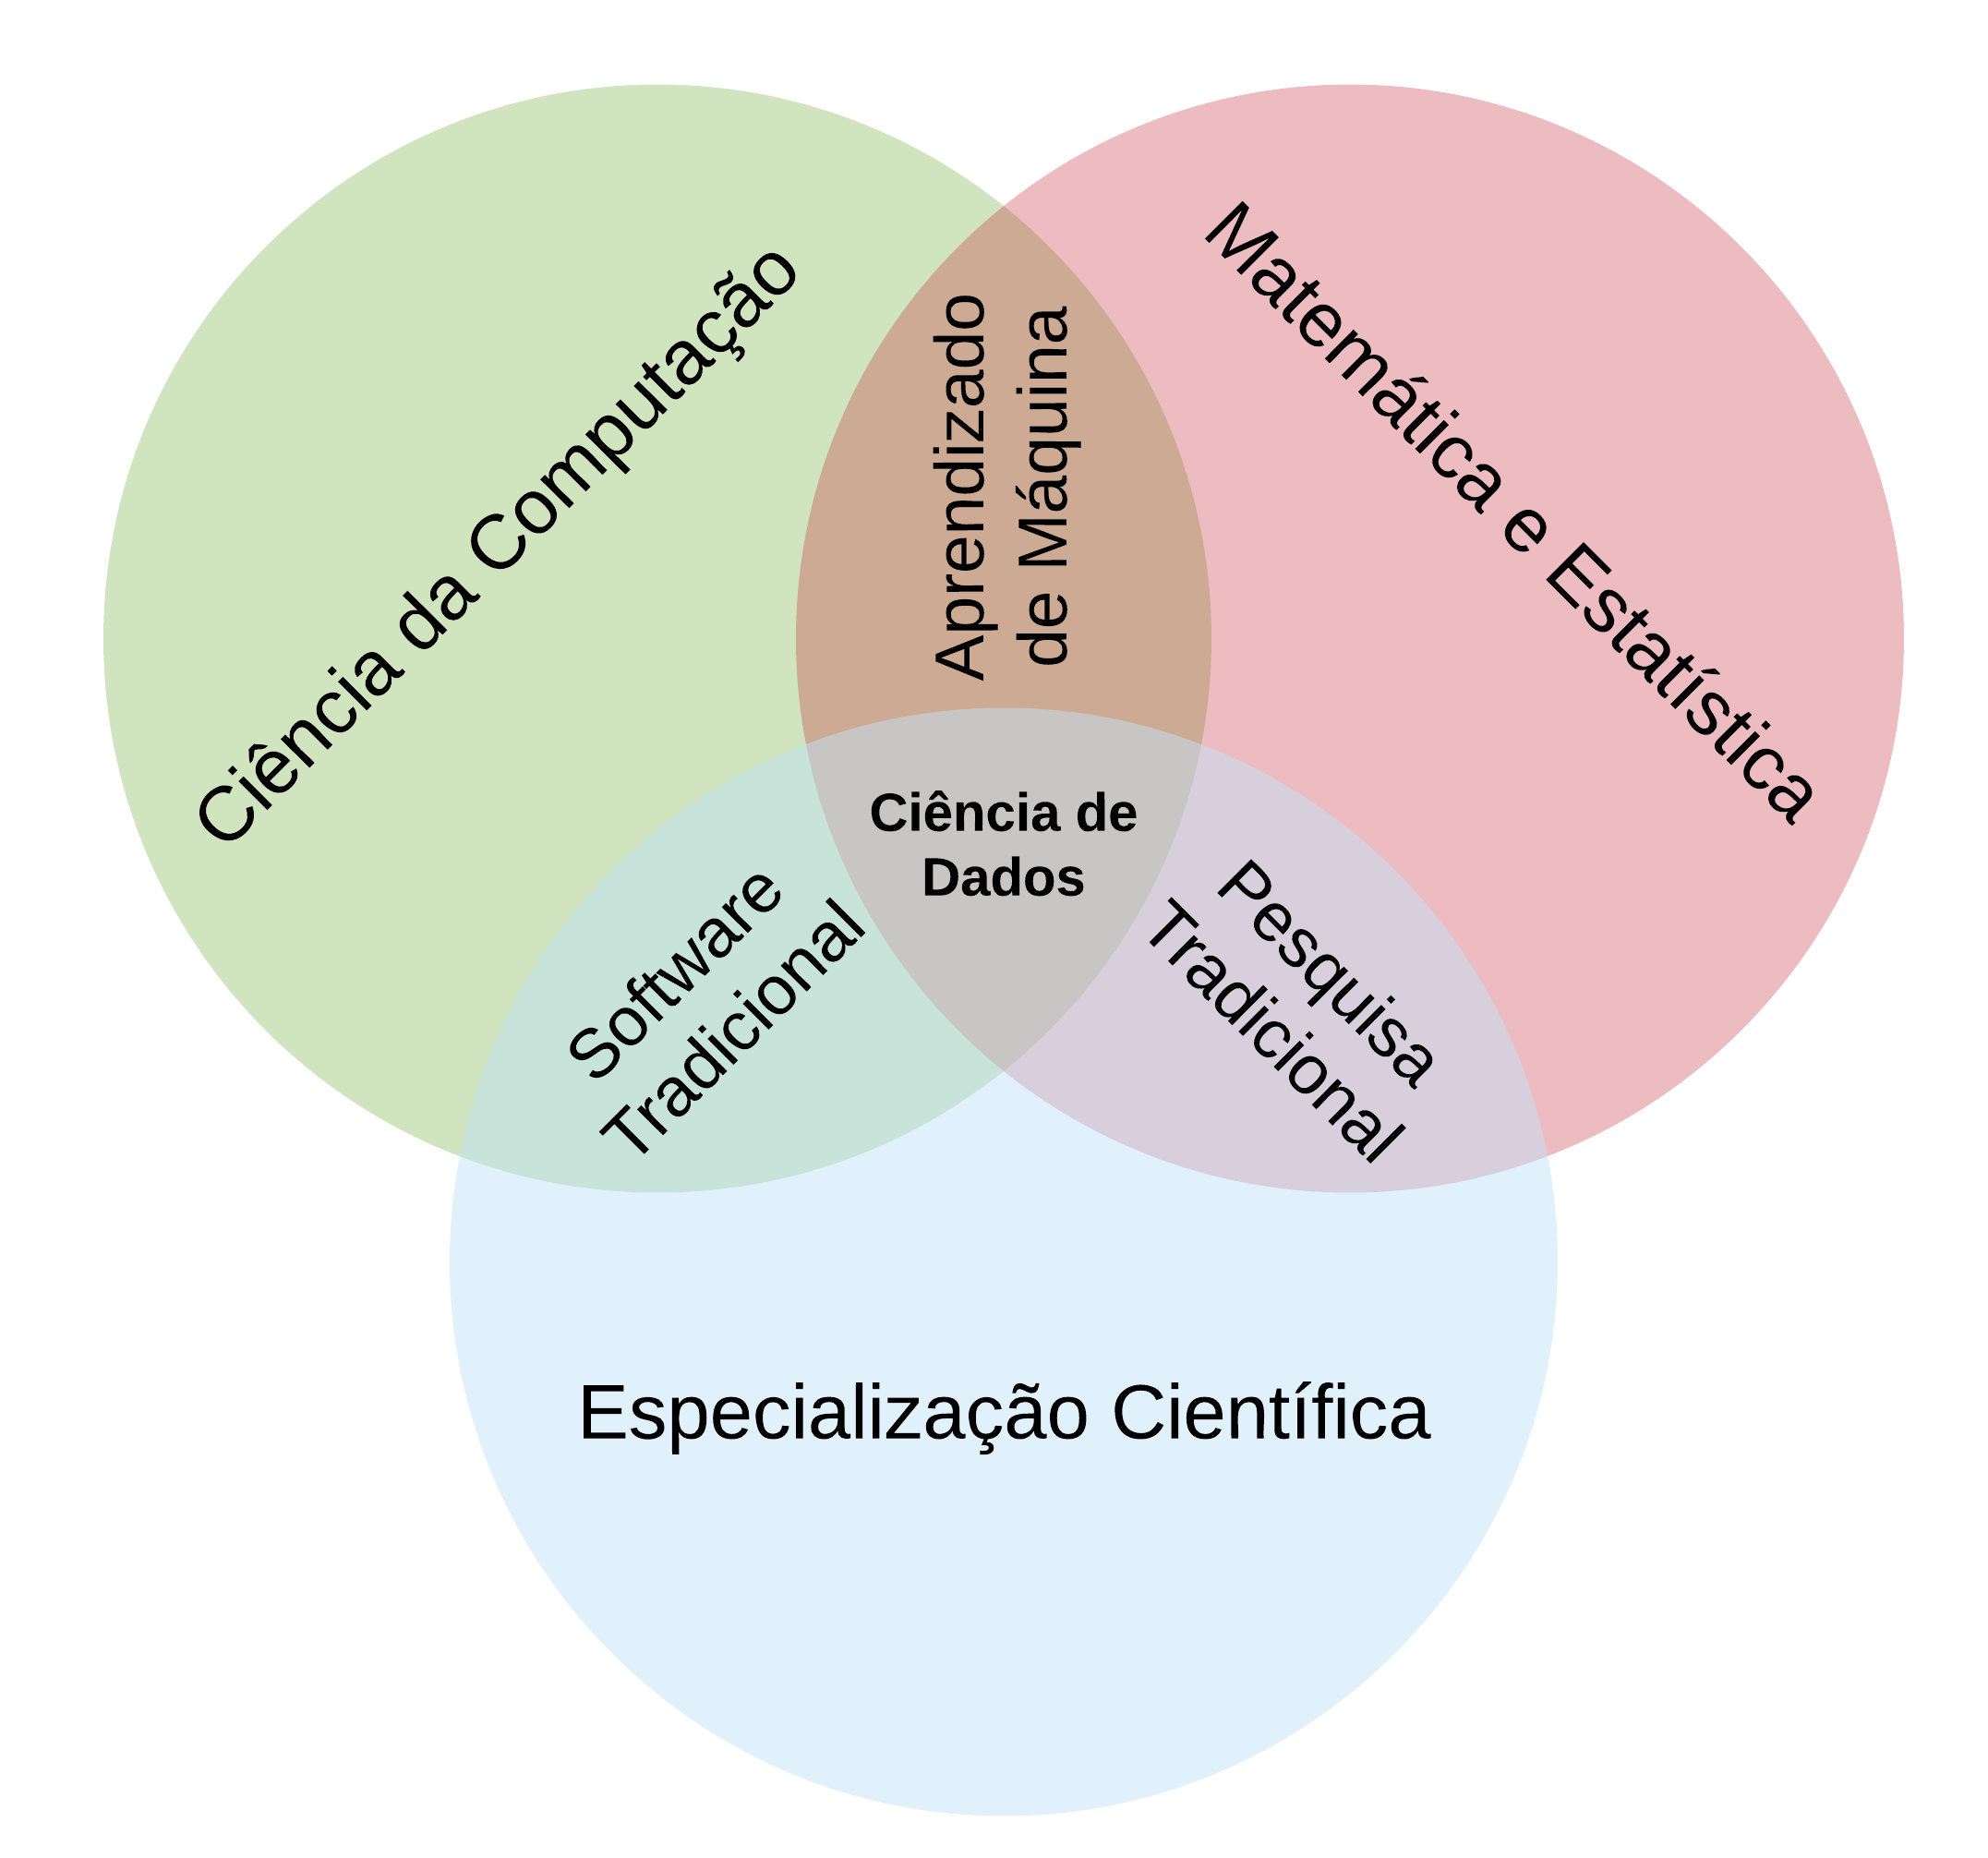
\includegraphics[width=0.55\textwidth]{figs/cap02_diagrama_veen_ds.png}
   \caption*{\footnotesize{Fonte: Adaptado de \cite{cap02_ref2}}}
   \label{fig:veen_diagram}
\end{figure}

A respeito da utilização de ciência de dados, a pesquisa de \cite{cap02_ref35} destaca que, embora o emprego de sistemas avançados de inteligência artificial mostre-se promissores em estratégias de negócios, a maioria das empresas não encontram-se preparadas para implementar tal abordagem. De acordo com a autora, há uma hierarquia de necessidades, nas quais, requisitos básicos necessitam ser atendidos antes de obter possíveis benefícios a partir da utilização de modelos de inteligência artificial. Contudo, destaca-se que a aplicação de análises estatísticas simples ou extração de características acerca dados sem representatividade podem ser compreendidas como aplicações da ciência de dados. 

Embora as principais aplicações da ciência de dados estejam fortemente relacionadas ao setor econômico e financeiro, devido principalmente ao fato de ter nascido neste ambiente para a resolução da problemática de grande quantidade de dados geradas pelas empresas \cite{cap02_ref9}, a utilização desta área nos desafios encontrados pela pesquisa científica tornou-se uma alternativa plausível em virtude, essencialmente, da sua capacidade adaptativa e interdisciplinar \cite{cap02_ref2}.

% --------------------------------------------------------------------------- %
\section{Dados Abertos}

O conceito de dados abertos, do inglês \textit{open data}¸ faz referência a dados que podem ser utilizados, reutilizados ou redistribuídos livremente por qualquer pessoa, restringindo, no máximo, a atribuição à fonte original e ao compartilhamento das mesmas licenças em que as informações foram apresentadas \cite{cap02_ref25}. Dessa forma, a abertura de dados objetiva restringir o controle e restrições existentes em dados que forem publicados, possibilitando a exploração dos seus conteúdos de forma livre por pessoas (sejam essas físicas ou jurídicas) \cite{cap02_ref24}. 

Assim sendo, em \cite{cap02_ref26} o conceito de dados abertos é compreendido por três normas fundamentais:

\begin{itemize}
    \item Os dados devem ser disponibilizados em um meio acessível, preferencialmente na internet, em um formato compreensível por máquina de tal forma que este possa ser acessado e modificado.
    
    \item Os dados devem ser disponibilizados perante a termos que permitam sua reutilização e redistribuição, inclusive a combinando com outros conjuntos de dados.
    
    \item Todos os usuários devem ser capazes de utilizar, reutilizar e redistribuir os dados, sem haver discriminação com áreas de atuação, pessoas ou grupos.
\end{itemize}

Uma vez que o movimento de dados abertos é estimulado e que as três regras supracitadas são atendidas, é aberta a possibilidade que diferentes pessoas, organizações e sistemas trabalhem de forma colaborativa. Tal fator é justificado pela interoperação dos dados que foram abertos, ampliando a comunicação existente e potencializando o desenvolvimento de sistemas cada vez mais complexos \cite{cap02_ref24}.

É importante ressaltar que os dados abertos não correspondem somente aqueles divulgados pelo governo, podendo originar de qualquer instituição contanto que atenda os requisitos básicos citados anteriormente, não apresentando restrições de uso \cite{cap02_ref37}. Existem casos de dados abertos disponibilizados por diversas industrias ou setores, como transporte, produtos, sustentabilidade, mapas, economia, cultura, finanças, negócios, entre outros. A Figura~\ref{fig:dadosabertos} apresenta alguns exemplos de tipos de dados abertos comumente encontrados na internet \cite{cap02_ref36}.

\begin{figure}[!h]
   \centering
   \caption{Tipos de dados abertos}
   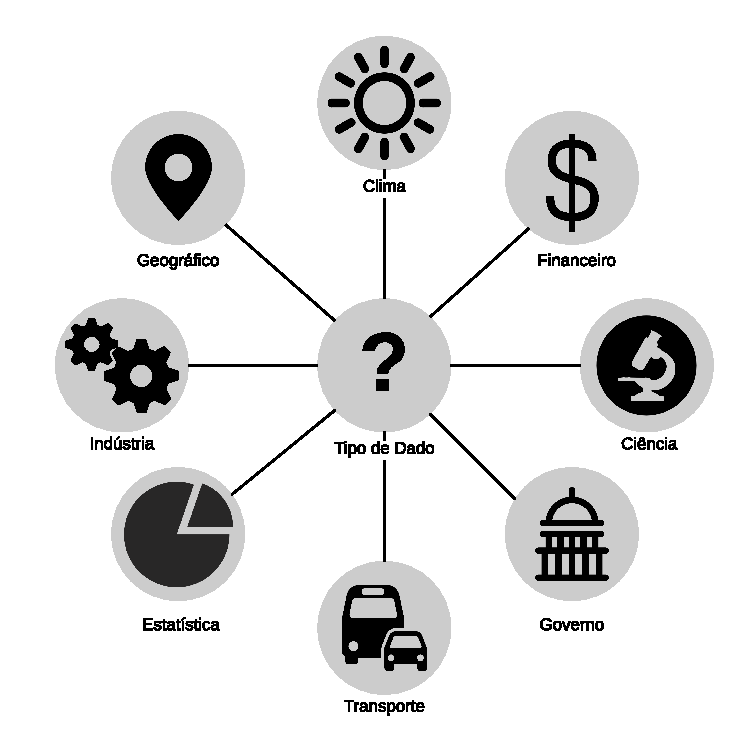
\includegraphics[width=0.75\textwidth]{figs/cap02_dados_abertos.pdf}
   \caption*{\footnotesize{Fonte: Adaptado de \cite{cap02_ref36}}}
   \label{fig:dadosabertos}
\end{figure}

\subsection{Dados Abertos Governamentais}

O conceito de dados abertos governamentais está sendo cada vez mais disseminado, sobretudo após a divulgação de um memorando em 2008 do até então presidente dos Estados Unidos Barack Obama \cite{cap02_ref27}. Neste, é discutida a transparência de dados governamentais norte-americanos através da criação de uma plataforma web \cite{cap02_ref28} que disponibilizasse dados abertos para qualquer cidadão.

A abertura dos dados públicos objetiva, sobretudo, estimular que a sociedade desenvolva produtos, serviços e novas atividades econômicas utilizando essas informações. Além disso, destacam-se benefícios políticos relacionados, principalmente, a transparência governamental gerada através do acompanhamento das elaborações de políticas públicas. Tal fator, além de intensificar a responsabilidade e participação democrática dos cidadãos, aumenta a confiabilidade transmitida pelo governo \cite{cap02_ref38}.

Nesse cenário, o governo brasileiro apresenta-se como um dos fundadores do \textit{Open Government Partnership} \cite{cap02_ref30} em 2011, uma iniciativa internacional que visa a promoção de governos abertos através da capacitação de cidadãos, combate a corrupção e aproveitamento de novas tecnologias. Além disso, a política de dados abertos governamentais no Brasil é consolidada pela Lei n. 12.527 de 2011, conhecida como Lei de Acesso à Informação (LAI), a qual garante acesso a qualquer informação de interesse público, desde que esta não seja imprescindível a segurança da sociedade e do Estado \cite{cap02_ref31}. De maneira similar aos Estados Unidos, no Brasil há uma plataforma de acesso aos dados abertos governamentais \cite{cap02_ref29}, sendo um portal que disponibiliza informações públicas seguindo os princípios de dados abertos relatados anteriormente.

No entanto, embora os dados abertos governamentais apresentem impactos extremamente positivos no governo, na sociedade e na economia, evidenciam-se adversidades relacionadas a sua implantação. Nesse contexto, o trabalho de \cite{cap02_ref38} divide esses obstáculos em seis grandes grupos: institucionais, complexidade da tarefa, utilização, legislação, qualidade da informação e técnicas. Dessa forma, a estimulação para a participação da população no uso dessas fontes de informações apresenta-se potencialmente promissora acerca das vantagens abordadas nessa subseção.

% --------------------------------------------------------------------------- %
\section{Técnicas Matemáticas Utilizadas}
\subsection{Decomposição do Índice de Gini}\label{cap:referencias:gini}

O índice de Gini, também conhecido como coeficiente de Gini, é uma medida de dispersão estatística elaborado pelo italiano Corrando Gini que objetiva mensurar o grau de desigualdade de uma variável acerca de um conjunto de dados \cite{cap02_ref19, cap02_ref20}. Esse indicador é fortemente utilizado em econômica para aferir o grau de desigualdade de renda da população, no entanto, é possível aplicá-lo em diversos campos de estudo como educação, ecologia, ciências da saúde, sociologia, dentre outros \cite{cap02_ref23}. Sua interpretação baseia-se em um número variado entre 0 e 1, no qual 0 corresponde a total igualdade (todos recebem a mesma renda) e 1 a total desigualdade (uma pessoa detém de toda renda e os demais nada) \cite{cap02_ref19, cap02_ref21}.

Matematicamente, assume-se uma série discreta $x_i (i, ..., n)$ correspondente a renda da $i$-ésima pessoa de uma população com $n$ pessoas. Admite-se que as rendas estão ordenadas, sendo:

\begin{equation} 
    x_1 \leq x_2 \leq ... \leq x_i \leq ... \leq x_n
    \label{eq:2.1}
\end{equation}

Agregando as pessoas da mais pobre até a i-ésima posição da série~\ref{eq:2.1}, a proporção acumulada da população é dada por:

\begin{equation}
    p_{i} = \frac{i}{n}
\end{equation}

\noindent e a respectiva para proporção acumulada de renda é:

\begin{equation}
    \varphi_i = \frac{1}{n \mu} \sum_{j=1}^{i} x_j
\end{equation}

\noindent onde $\mu$ é a renda média, dada por:

\begin{equation}
    \mu = \frac{1}{n} \sum_{i=1}^{n} x_i
\end{equation}

A Curva de Lorenz é obtida pela relação entre os pares ordenados dos valores de $p_i$ e $\varphi_i$, conforme indicado na Figura~\ref{fig:lorenz_curve}.

\begin{figure}[!h]
   \centering
   \caption{Curva de Lorenz}
   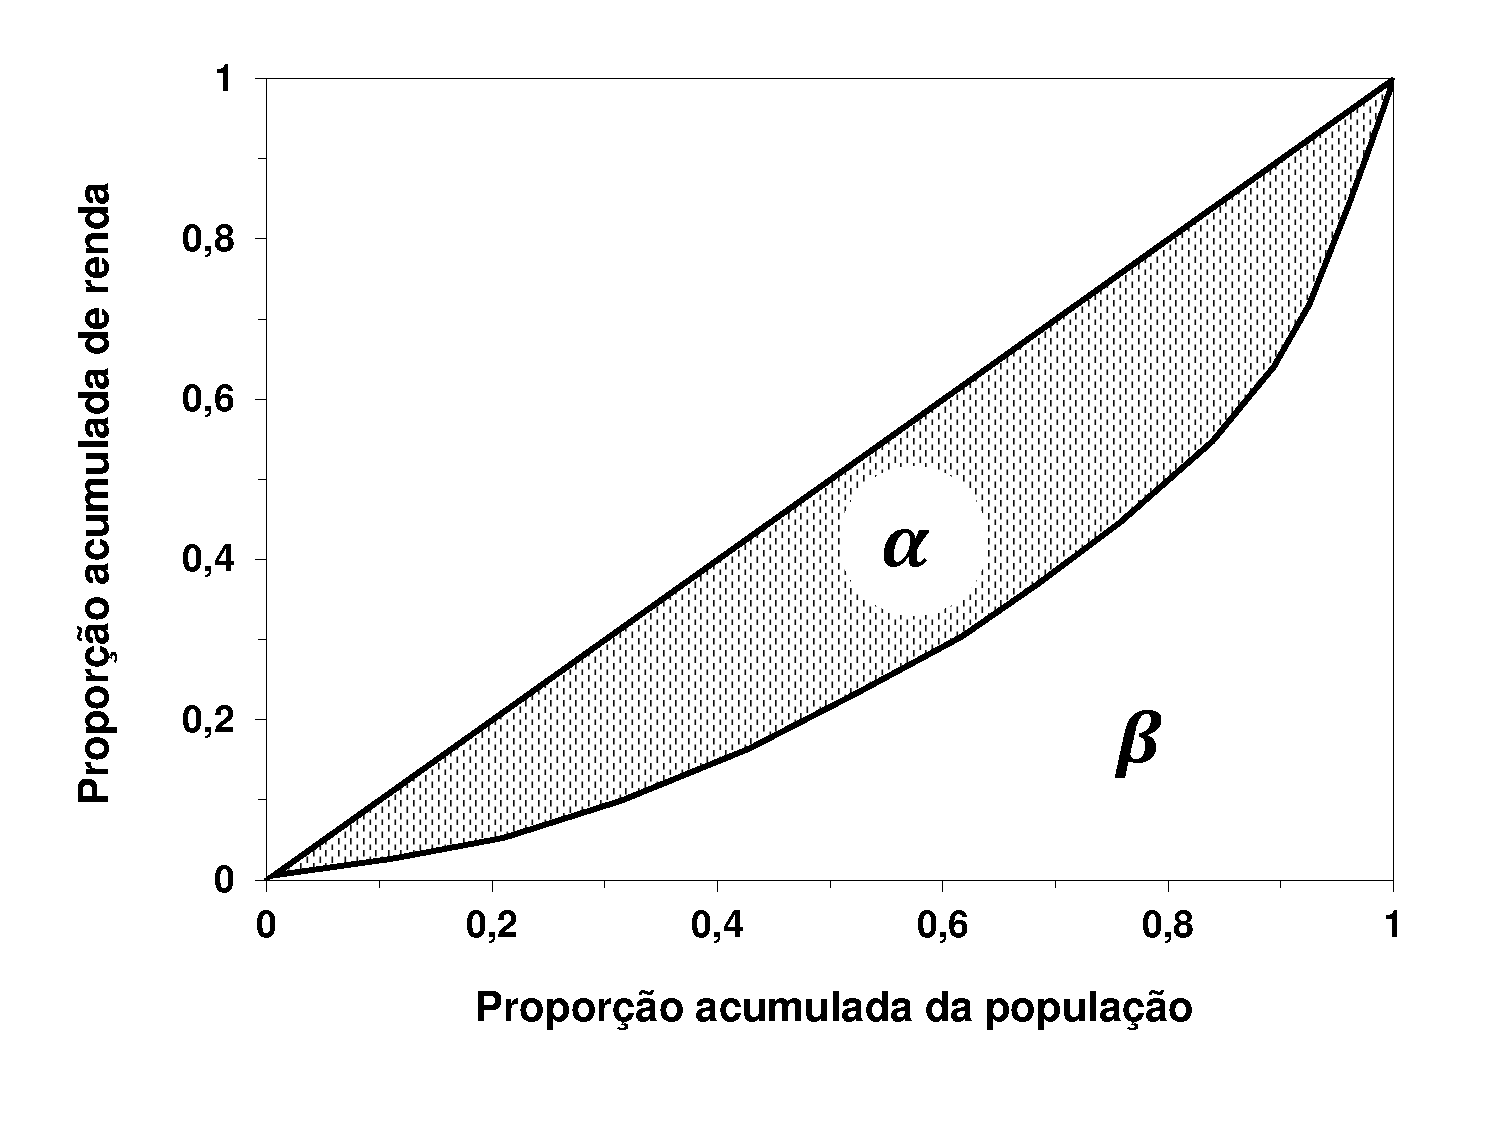
\includegraphics[width=0.8\textwidth]{figs/cap02_curva_lorenz.pdf}
   \caption*{\footnotesize{Fonte: Adaptado de \cite{cap02_ref20}}}
   \label{fig:lorenz_curve}
\end{figure}

O coeficiente de Gini corresponde ao quociente da área $\alpha$ com a soma das áreas $\beta$ e $\alpha$, ou seja: 

\begin{equation}
    G = \frac{\alpha}{\alpha + \beta} = \frac{\alpha}{0,5}
    \label{eq:2.5}
\end{equation}

Dessa forma pode-se reescrever a equação~\ref{eq:2.5} como:

\begin{equation}
    G = 1 - 2\beta
    \label{eq:2.6}
\end{equation}

Similarmente, é possível considerar que a renda $x_i$ é composta por $k$ parcelas de rendimento de forma que: 

\begin{equation}
    x_i = \sum_{h=1}^{k}x_{hi}
\end{equation}

\noindent onde $x_{hi}$ representa o valor da $h$-ésima parcela de renda da $i$-ésima pessoa. Sendo assim, a média da $h$-ésima parcela é:

\begin{equation}
    \mu_h = \frac{1}{n} \sum_{i=1}^{n}x_{hi}
\end{equation}

\noindent e a proporção acumulada dessa parcela referente a série~\ref{eq:2.1} é dado por:

\begin{equation}
    \varphi_{hi} = \frac{1}{n\mu_h} \sum_{j=1}^{i} x_{hj}
\end{equation}

Analogamente a equação~\ref{eq:2.6} é possível definir a curva de concentração como sendo a relação dos pares ordenados de $\varphi_{hi}$ e $p_i$. Ressalta-se que na construção da curva de concentração de $x_{hi}$ é utilizada a ordenação de $x_i$ e não a ordenação de $x_{hi}$, que pode ser diferente. Sendo assim, do mesmo modo que para o coeficiente de Gini, define-se a Razão de Concentração da parcela $h$ $(C_h)$ como:

\begin{equation}
	C_h = 1 - 2\beta_h
	\label{eq:2.10}
\end{equation}

\noindent onde $\beta_h$ é a área entre a curva de concentração de $x_{hi}$ e o eixo das abscissas.

Diante disso, \cite{cap02_ref22} demonstra que o índice de Gini é definido pela média ponderada das razões de concentração das parcelas $h$. Então:

\begin{equation}
	G = \sum_{h=1}^{k} \varphi_h C_h
\end{equation}

\noindent como $\sum_{h=1}^{} \varphi_h = 1$, pode-se reescrever a equação 1 como:

\begin{equation}
	G = G - \sum_{h=1}^{k} \varphi_h (G - C_h)
\end{equation}

\noindent com, 

\begin{equation}
	\pi_h = G - C_h
	\label{eq:2.13}
\end{equation}

A equação~\ref{eq:2.13} é conhecida como medida de progressividade, na qual $\pi_h > 0$ ($C_h < G$) simboliza uma parcela progressiva (contribuindo para o decréscimo do índice de Gini e diminuição da concentração de renda). De forma semelhante $\pi_h < 0$ ($C_h > G$) corresponde a uma parcela regressiva (contribuindo para o acréscimo do índice de Gini e aumentando a concentração de renda) \cite{cap02_ref22}.

\subsection{Correlação de Variáveis}\label{cap:referencias:correlacao}

Em estatística, correlação compreender a interdependência existente entre duas variáveis, ou seja, o grau de relacionamento ou associação existentes entre as características de um dado. Em alguns casos essa relação é clara, como a massa corporal e a altura de uma pessoa, o consumo de combustível e a distância percorrida por um veículo ou o número de anúncios divulgados e a quantidade de produtos vendidos. Todavia, em muitos casos essa interdependência não é intuitiva ou aparente, fazendo necessário, dessa forma, a utilização de estratégias matemáticas para aferir essa correlação \cite{cap02_ref39}. Dentre os métodos mais comuns temos os índices de Pearson, Spearman e Kendall.

O coeficiente de correlação de Pearson, também conhecido como coeficiente de correlação produto-momento, é responsável por mensurar a interdependência, positiva ou negativa, existente entre duas variáveis. Essa estimativa, normalmente representada por $\rho$, assume valores entre -1 e 1, onde 1 corresponde a uma correlação perfeita positiva entre as variáveis, e -1 a uma correlação perfeita negativa, ou seja, se uma aumenta a outra sempre diminui. Por outro lado, quando o valor de $\rho$ é igual 0 observa-se uma interdependência linear entre as variáveis, podendo, no entanto, existir uma dependência não-linear entre elas \cite{cap02_ref41, cap02_ref40}.

O cálculo do coeficiente de correlação de Pearson pode ser realizado a partir da seguinte fórmula: 

\begin{equation}
    \rho = \frac{cov(X,Y)}{\sqrt{var(X).var(Y)}} = \frac{\sum_{i=1}^{n} (x_{i} - \bar{x})(y_{i} - \bar{y})} {\sqrt{\sum_{i=1}^{n} (x_{i} - \bar{x})^2} . \sqrt{\sum_{i=1}^{n} (y_{i} - \bar{y})^2}}
    \label{eq:2.14}
\end{equation}

\noindent onde, $x_{1}, x_{2}, ..., x_{n}$ e $y_{1}, y_{2}, ..., y_{n}$ correspondem aos valores assumidos por cada variável, e $\bar{x}$ e $\bar{y}$ são suas respectivas médias aritméticas.

A correlação de Pearson mensura a associação linear entre variáveis contínuas, estimando o quanto a relação dessas variáveis pode ser descrita por uma reta \cite{cap02_ref41}. Diante disso, pode ser interpretar o valor de $\rho$ como:

\begin{itemize}
    \item 0,9 a 1 positivo ou negativo indica uma correlação muito forte.
    \item 0.7 a 0.9 positivo ou negativo indica uma correlação forte.
    \item 0.5 a 0.7 positivo ou negativo indica uma correlação moderada.
    \item 0.3 a 0.5 positivo ou negativo indica uma correlação fraca.
    \item 0 a 0.3 positivo ou negativo indica uma correlação desprezível.
\end{itemize}

De maneira similar, o coeficiente de Spearman é comumente utilizado para aferir a interdependência existente entre variáveis aleatórias relacionadas monotonicamente\footnote{Uma função entre dois conjuntos de dados é considerada monótona quando há a preservação da relação de ordem no seu domínio.}, mas não de maneira linear. A forma deste coeficiente de correlação é a mesma do coeficiente de Pearson, mas as variáveis não correspondem mais aos valores originais coletados, substituindo-os por postos correspondes ao valor que cada variável assume em uma ordenação numérica \cite{cap02_ref39}.

O coeficiente de correlação de Spearman pode ser aferido da seguinte forma: 

\begin{equation}
    \rho = 1 - \frac{6 \ \mathlarger{\sum_{i-1}^{n}} \ (X - Y)^2}{n(n^2 - 1)}
    \label{eq:2.15}
\end{equation}

\noindent onde $X$ e $Y$ são as variáveis aleatórias variando de 1 a $n$, com $n$ sendo a quantidade de elementos existentes no conjunto.

O coeficiente de Kendall, por sua vez, avalia a interdependência de postos ordenados, semelhante a correlação de Spearman. Essa medida é comumente eficiente para dados discretos, na qual $\left(x_1, y_1\right)$, $\left(x_2, y_2\right)$, ..., $\left(x_n, y_n\right)$ compreendem conjuntos de observações das variáveis aleatórias $X$ e $Y$, tal que $x_i$ e $y_i$ sejam valores únicos. Qualquer par ordenado de observações, em que $i\ \neq\ j$, é considerado concordante se as classificações dos elementos concordarem entre si, ou seja, se $x_i > x_j$ e $y_i > y_j$, ou se $x_i < x_j$ e $y_i < y_j$. De maneira similar, eles serão discordantes se $x_i > x_j$ e $y_i < y_j$, ou se $x_i > x_j$ e $y_i < y_j$. Na hipótese de $x_i = x_j$ e $y_i = y_j$, o par não será nem concordante e nem discordante \cite{cap02_ref42, cap02_ref39}. Dessa forma, é possível calcular o coeficiente de correlação de Kendall $(\tau)$ conforme a Equação~\ref{eq:2.16}:

\begin{equation}
    \tau = \frac{(quantidade \ de \ pares \ concordantes) - (quantidade \ de \ pares \ discordantes)}{n(n - 1)/2}
    \label{eq:2.16}
\end{equation}

É importante destacar que a correlação não indica necessariamente causa. Por exemplo, considere um estudante que teve boas notas nas disciplinas de química e física. O bom desempenho em química não pode ser necessariamente atribuído ao bom desempenho em física, mas ambas as notas podem ser explicas por um bom desempenho em matemática, fator não considerado no primeiro momento. Dessa forma, a correlação apresenta-se como uma importante ferramenta para análise de dados uma vez que, quando interpretada corretamente, possibilita a abstração de informações relevantes acerca de conjuntos de atributos interdependentes.

% --------------------------------------------------------------------------- %
\section{Considerações Finais}

Nesse capítulo foi apresentada a fundamentação teórica que norteou o desenvolvimento desta dissertação, iniciando por uma contextualização acerca de análise de dados, a qual evidenciou o conceito de processo de extração de conhecimento \cite{cap02_ref12} – relatando a sua diferença em relação a mineração de dados \cite{cap02_ref5} – e suas aplicações no cenário empresarial a partir do método de BI \cite{cap02_ref15, cap02_ref16}. Com base nessas definições, foi realizada a conceituação de ciência de dados \cite{cap02_ref9, cap02_ref1, cap02_ref3}, relatando sua relevância perante o atual cenário de produção de informações \cite{cap02_ref4} e evidenciando sua capacidade adaptativa de trafegar entre as diversas áreas de conhecimento \cite{cap02_ref2}.

Posteriormente, foi apresentado o conceito de dados abertos destacando sua importância nos mais diversos campos como ferramenta de acesso a informação para a sociedade \cite{cap02_ref4}. Nesse âmbito, enfatizou-se os dados abertos governamentais como mecanismo para a disponibilização de conteúdo público para a população, objetivando oferecer um sistema governamental mais transparente tanto no Brasil como em diversos países do mundo \cite{cap02_ref25}.

Por fim, foram conceituadas algumas das técnicas matemáticas utilizadas nesta pesquisa. Primeiramente, fez-se uma definição acerca da decomposição do coeficiente de Gini \cite{cap02_ref19}, destacando sua utilização para aferir o grau de desigualdade de uma população acerca de uma determinada variável, como por exemplo a seu rendimentom e sua capacidade de mensurar o quanto cada parcela dessa variável influencia para diminuir ou aumentar a desigualdade existente. Em seguida, foram detalhados os conceitos de correlação entre variáveis interdependes, enfatizando sua eficiência para abstração de informação útil acerca de atributos em conjuntos de dados \cite{cap02_ref39}.
